% Intended LaTeX compiler: pdflatex
\documentclass{scrartcl}
<<<<<<< HEAD
    \usepackage[utf8]{inputenc}
    \usepackage[dvipdfmx]{color}
    \usepackage[backend=biber,bibencoding=utf8]{biblatex}
    \usepackage{url}
    \usepackage{indentfirst}
    \usepackage[normalem]{ulem}
    \usepackage[dvipdfmx]{hyperref}
    \usepackage{longtable}
    \usepackage{minted}
    \usepackage{fancyvrb}
    \usepackage[dvipdfmx]{graphicx}
    \usepackage[top=25truemm,bottom=25truemm,left=25truemm,right=25truemm]{geometry}
    \bibliography{reference}
\author{情報科学類二年 江畑 拓哉(201611350)}
\date{}
\title{seis-ml-api中間レポート2}
=======
		\usepackage[utf8]{inputenc}
		\usepackage[dvipdfmx]{graphicx}
		\usepackage[dvipdfmx]{color}
		\usepackage[backend=biber,bibencoding=utf8]{biblatex}
		\usepackage{url}
		\usepackage{indentfirst}
		\usepackage[normalem]{ulem}
		\usepackage{longtable}
		\usepackage{minted}
		\usepackage{fancyvrb}
    \usepackage[dvipdfmx,colorlinks=false,pdfborder={0 0 0}]{hyperref}
    \usepackage{pxjahyper}
		\bibliography{reference}
\author{情報科学類二年 江畑 拓哉(201611350)}
\date{}
\title{seis-ml-api中間レポート(再編)}
>>>>>>> 8b06f277a20cc3d6e2ac8260de58bd4f3f6fca06
\begin{document}

\maketitle
\tableofcontents


<<<<<<< HEAD
\section{情報特別演習概要}
\label{sec:org9f80ab5}
 本演習は江畑、栗本、畑中の3名により実施する。それぞれ演習を進め、最終的に大規模データベースを用いた機械学習API(seis-ml-api)を作成することが目標である。\\

\subsection{演習範囲に関して}
\label{sec:org40df129}
 以下に示す範囲を演習し、その成果を組み合わせることでseis-ml-apiの作成を目指す。\\

\begin{table}[htbp]
\caption{演習範囲に関して}
=======
\section{前書き}
\label{sec:org470ddd7}
 このレポートは``江畑拓哉個人''が作成した情報特別演習における中間レポートである。ここで記載されているものは、現在までの成果を出した進捗に限り、それまでの失敗した試行などについては記載されていない。\\
 また既存のツールを用いて実験した結果や、機械学習やデータベースの細かいプログラムについては完成次第別紙に実験レポートに作成する。\\
 最後にこのレポートに関する意見などに関しては混乱を避けるため、できうる限り直接ご指摘頂ければ幸いである。\\
\section{seis-ml-api概要}
\label{sec:orgd866fc1}
 この api (と仮定する)は、この情報特別演習をグループで受講した我々(江畑,栗本,畑中)の最終的な目標である。我々はまず各々の学ぶ分野についての理解を深め、その成果を適宜持ち寄ってこれを作成する予定になっている。\\

\begin{table}[htbp]
\caption{主な役割について(但し互いに柔軟に協力し合う)}
>>>>>>> 8b06f277a20cc3d6e2ac8260de58bd4f3f6fca06
\centering
\begin{tabular}{|c|c|c|}
\hline
氏名 & 分野 & 内容\\
\hline
<<<<<<< HEAD
江畑 & データベースと機械学習の統合 & 大規模データを利用した機械学習の作成\\
\hline
栗本 & 機械学習 & 機械学習モデルの調整\\
\hline
畑中 & データベース & 大規模データベースの作成\\
=======
畑中 & データベース & 大規模データベースの作成\\
\hline
栗本 & 機械学習 & 機械学習の理解\\
\hline
江畑 & 上記2つの統合 & 大規模データと機械学習を利用する手法の学習\\
>>>>>>> 8b06f277a20cc3d6e2ac8260de58bd4f3f6fca06
\hline
\end{tabular}
\end{table}

<<<<<<< HEAD
\subsection{seis-ml-api概要}
\label{sec:orgd312151}
 seis-ml-apiは、機械学習を提供するWeb APIである。大規模データベースを採用する。\\
 seis-ml-apiのフローをに示す。\\

\begin{figure}[htbp]
\centering
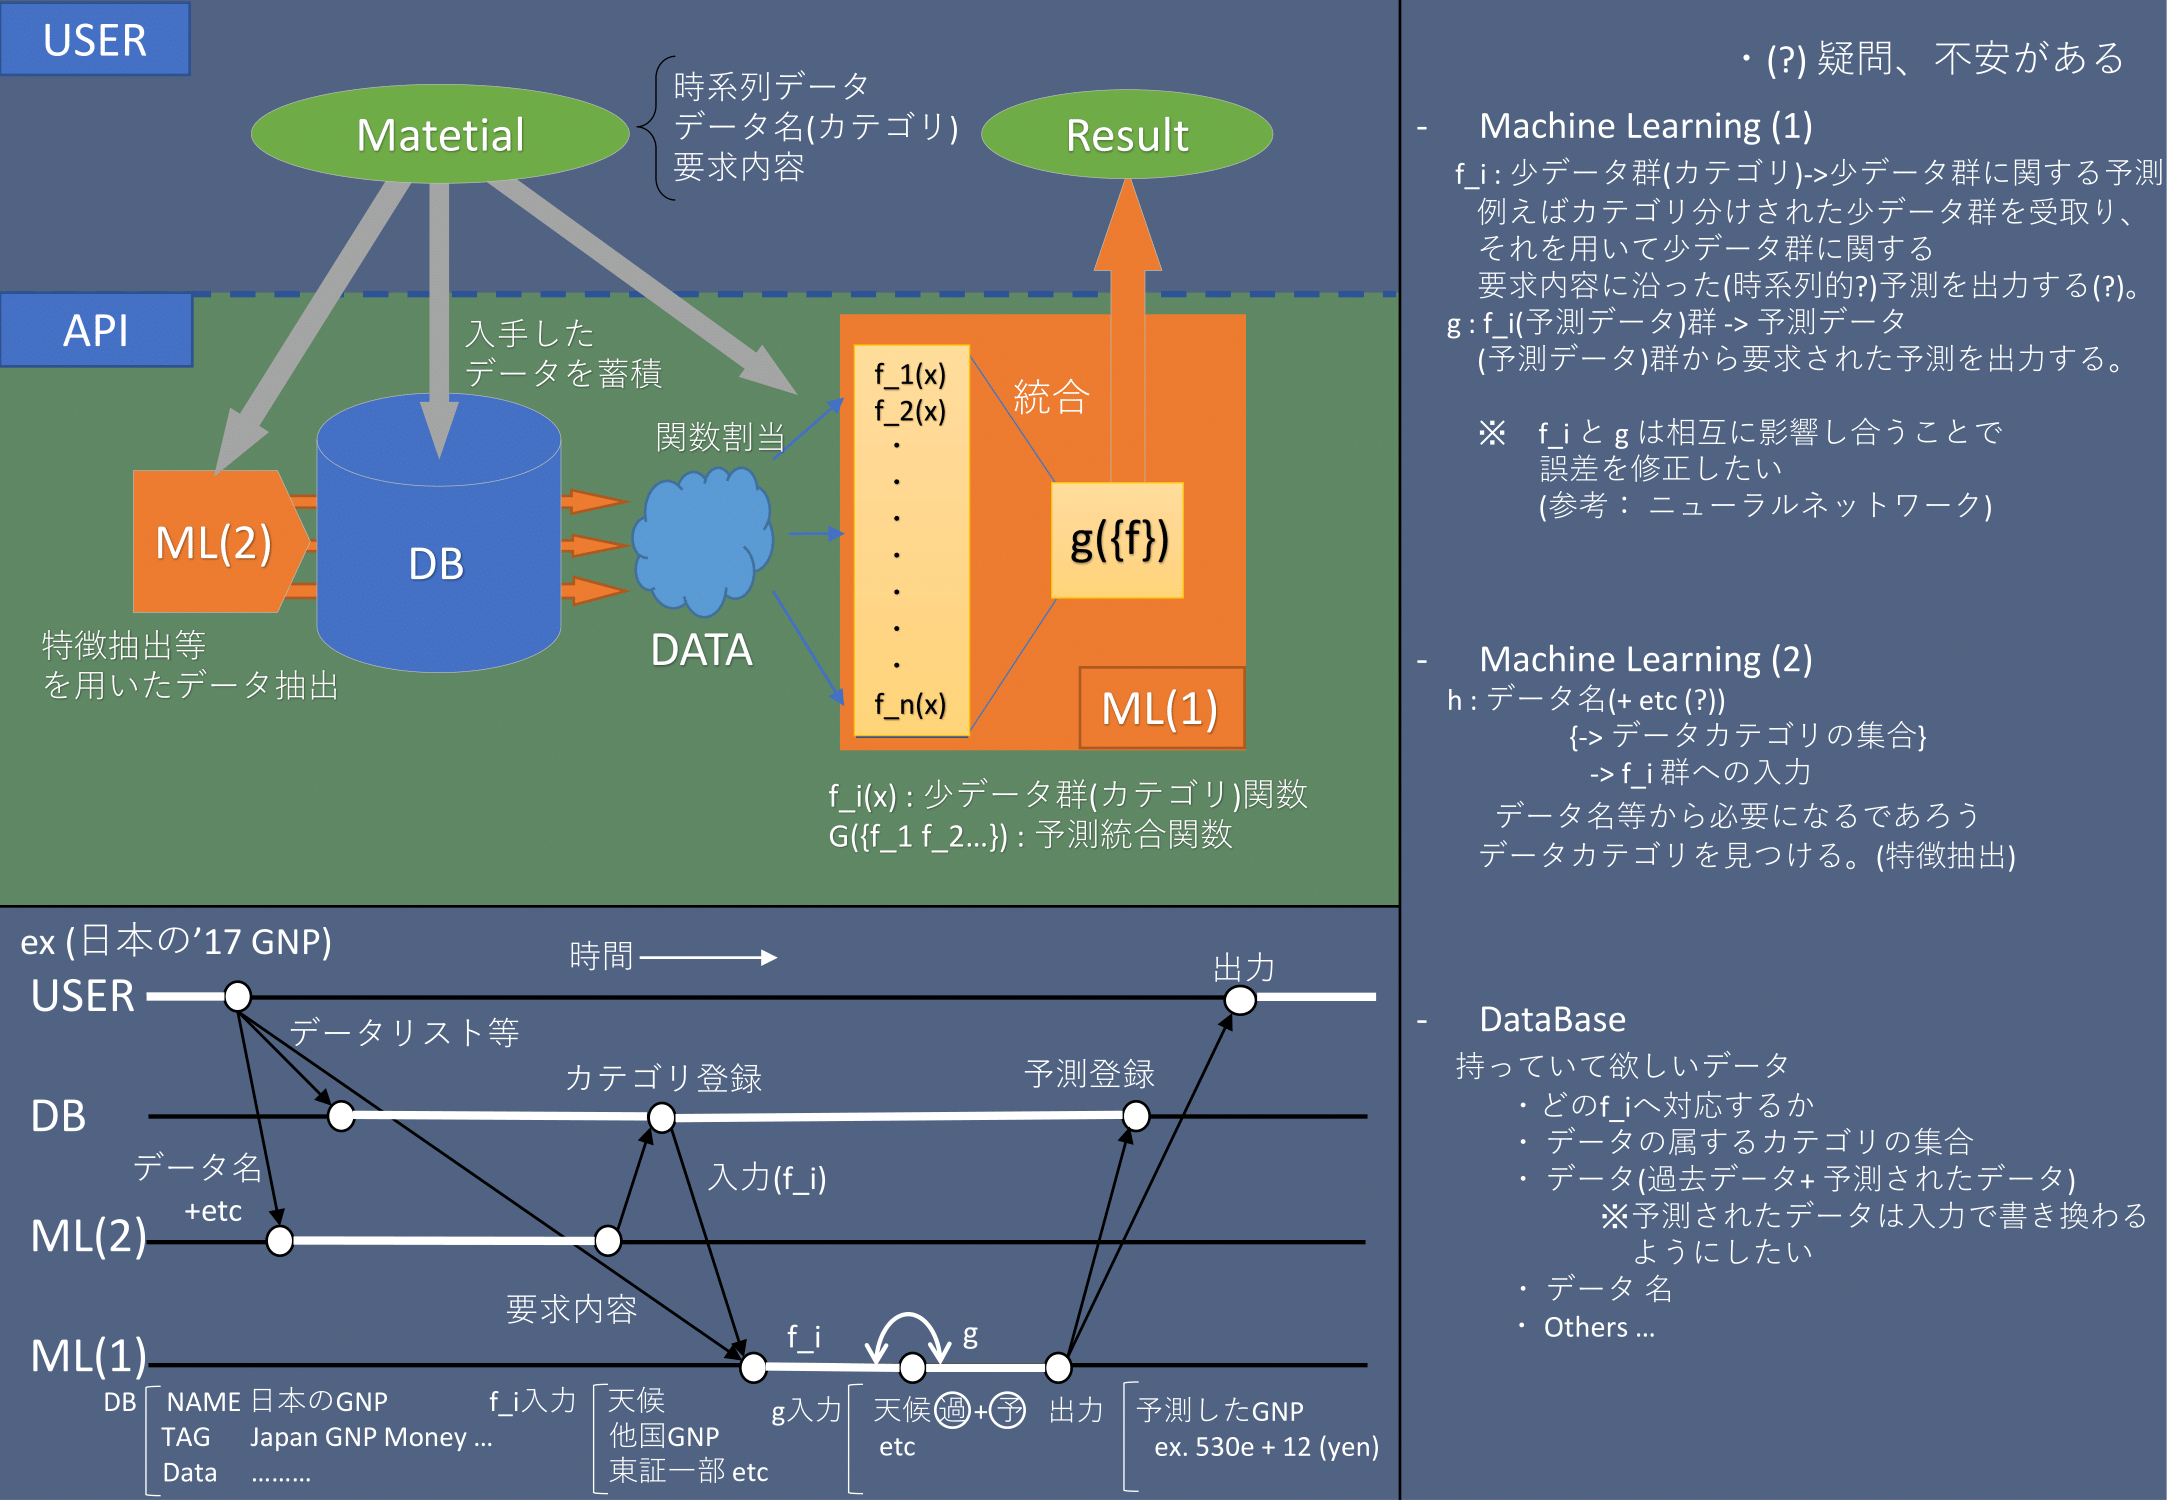
\includegraphics[width=15cm]{./idea-0-1.png}
\caption{seis-ml-api フロー}
\end{figure}

 ユーザはAPIに自分の持っているデータを登録する。APIは、APIに登録されているデータを用いて機械学習処理を行い、その結果をユーザに返す。\\

\subsection{実験に用いるデータ}
\label{sec:org3a61408}
 以下のデータをデータベースに登録し、実験段階においても用いたいと考えている。\\
   データの相関を求める関係上、これらの入手元から日本国内の経済についてのデータを集めたいと考えている。\\

\begin{itemize}
\item Quandl\\
 ほとんどすべてのデータはここで手に入る。ただし、長期間のデータは乏しいようである。主には、ここから得た株価データを用いて分析を行う予定である。\\
\item google finance\\
日本のデータをcsv形式で入手することは困難だが、海外のデータは容易に手に入る。\\
\item 総務省統計データ\\
 めぼしいデータは少ないが、ゼロではないため活用していきたい。\\
\end{itemize}

\section{それぞれの進捗について}
\label{sec:org4e0996c}
\begin{itemize}
\item 江畑\\
以下に引用されている文書を学習し、その結果より機械学習アルゴリズムの策定を行った。それに加え Java 、Python 、Clojure での Hbase の利用方法について学習した。\\
\item 栗本\\
「機械学習」の履修及び関連書籍の学習を行った。また、主専攻実験「ヒューマンセンシング」の自主実験において、サポートベクターマシンを用いた簡易画像分類器を作成した。\\
\item 畑中\\
HBase 、Hadoop を用いて疑似分散環境を構築した。また、JavaからHBaseにアクセスする方法を、実際にプログラムを動作させて確認した。\\
\end{itemize}


\section{今後の演習について}
\label{sec:orgf289936}
\begin{itemize}
\item 江畑\\
\end{itemize}
策定した機械学習のモデルを実際のコードに実現する作業とHBaseに入力されたデータを送るAPIを作成する。\\
\begin{itemize}
\item 栗本\\
\end{itemize}
機械学習モデルの理解を深め、Pythonによるデータ分析に慣れ、より良いモデル調整が可能なように学習していきたいと考えている。\\
\begin{itemize}
\item 畑中\\
\end{itemize}
 完全分散環境を構築して、HBaseの性能テストを行いたいと考えている。\\



\section{参考文献}
\label{sec:org413c898}
=======
 つまり、我々の情報特別演習のゴールは二段階あり、一段階はそれぞれの学習分野の習得、二段階はそれらを持ち寄ってこの seis-ml-api という何かの作成を行う、というものである。\\
 問題となる api の詳細についてだが、機械学習が何を返すことができるものであるのかを全員が共有できていないため、詳細な情報を明記することはできない。しかし目標を理解しやすくするため、無理にこれについて個人的な見解に基づいた説明を行う。\\
 この api では以下の抽象的なチャートに基づいた設計を行う予定である。\\

\begin{figure}[htbp]
\centering
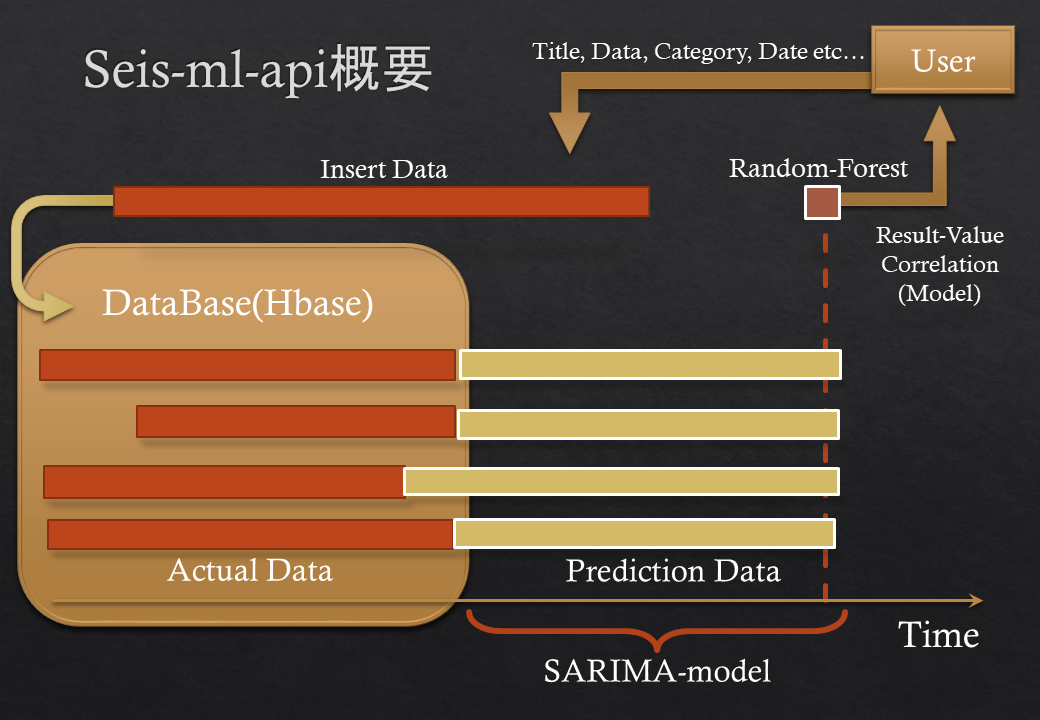
\includegraphics[width=15cm]{./idea-1.png}
\caption{seis-ml-apiの抽象的チャート}
\end{figure}

 ここで注意しなければならないのは、この案に関してはデータベースに Hbase を利用するという点以外に関しては江畑が独断で学習した成果によって作成されたものであり、機械学習分野のこれからの成果次第では作成されるものも、またこの制作物の利用法も十分に変わり得るということである。\\
 その前提に於いて、現在までのこの物の利用価値について説明するならば、恐らくこの api は``大量の時系列データを利用した価格予測api''と呼べるものなのではないだろうか。ユーザから時系列データを受取り、データベースに保存されたデータと関連付けて機械学習を行い、ユーザから指定された時点の予測値や相関の強いデータの名称を返す、というのが現時点での江畑の理解である。\\
 そしてこの構成要素は、大きく分けて機械学習とデータベースの二つである。\\
 データベースに関しては畑中氏が作成している、大規模データを扱うことのできる HBase を用いる予定である(詳細は彼と彼の担当の教員に尋ねて頂きたい)。江畑はこのデータベースに入手したデータ、それを予測したデータ、後述する SARIMA 予測をする際に用いるモデルなどを入れるつもりである。\\
 機械学習部分では、まず問題となる時系列データについてデータベースから関連性のあるデータを読み出し、それらについて時系列予測を行う。そしてそれらを元にして問題となった時系列データとの相関を調べ、いわば欠損値となっているユーザから指定された時点での値を求める。そしてその際に求まる相関の強かった関連データの名称も合わせてユーザに返すことが、この部分での実装予定のものである。\\
 \\
 これだけでは抽象的で理解が難しいため、江畑の考えている動作の流れを以下に示す。\\
 例えばユーザから、現在までのある時系列データがそれの所属するカテゴリ付きで渡されたとする。まずデータベース側から、指定されたカテゴリに関する時系列データ群が機械学習側に渡される。機械学習側ではそれらをユーザから指定された時点(例えば一週間後)まで時系列予測する。次にユーザから渡されたデータに対して先ほど予測したデータ群との相関を求めていく。その相関を用いて指定された時点の値を予測する。結果としてその値と相関の強かったデータの名称群を返す。最後にユーザから渡されたデータをデータベース側に保存して一連の動作は終了となる。\\

つまり必要となるデータは、\\
\begin{itemize}
\item タイトル\\
\item 時系列データ\\
\item そのデータの属するカテゴリ\\
\item 欲しい時点についての情報\\
\end{itemize}

 そして返すデータは、\\
\begin{itemize}
\item 予測値\\
\item 相関についてのデータ\\
\end{itemize}

 ということになる。\\

\subsection{実験に用いるデータ}
\label{sec:orgcfaae24}
 ここでは、初期にデータベースに入っているデータとして挙げられ、なおかつ実験段階に於いて使用できると考えられるデータの入手元について紹介する。江畑個人の考えとしては、データの相関を求める関係上、これらの入手元から日本国内の経済についてのデータを集めて行きたいと考えている。\\
\begin{itemize}
\item google finance\\
日本のデータをcsvで入手することは困難だが、海外のデータは容易に手に入る。\\
\item Quandl\\
 ほとんどすべてのデータはここで手に入る。但し、どうやら長期間のデータは乏しいようである。主にはこちらから得た株価データを用いて解析を行う予定である。\\
\item 総務省統計データ\\
 あまりめぼしいデータはないが、ゼロというわけではないため活用していきたいと考えている。\\
\end{itemize}

\section{機械学習部分(時系列解析)}
\label{sec:org5f136a4}
  この章に関する内容は全て江畑個人の報告であり、他のメンバーの活動に何ら影響を与えるものではない。\\
 実験に関しては、別紙にまとめて示す。(仮決定のこの部分のみの実験データは同フォルダのreport.ipynbである)\\
 時系列解析に用いるモデルは、季節的自己回帰和分移動平均モデルことSARIMAモデルを用いる予定である。\\
 SARIMAモデルとは、三つの要素が重ね合わさったモデルである。\\
 まずARという部分は Autoregressive を表し、これは自己回帰を意味する。内容は自分の以前の観測データに対して重回帰分析を行うというものである。例えば、 \(a->b->c\) という遷移があれば、 \(b->c->d\) といったことを考えられることに似ている。\\
 MAというのは Moving average 、つまり移動平均を意味している。移動平均とは、ある区間 [a, b] の平均値と b 或いは a などを比較する際に用いられる言葉のようで、平均値を平均の位置ではない別の位置の値と比較することを意味している。\\
 ARIMAというのは、以上の2つを組み合わせるという意味である。\\
 そしてSというのは、Seasonal、季節性という意味で、ある期間の周期性を用いるということである。これは例えば毎年同じような活動をするものに対して非常に有効な手段であるようで、 ARIMA モデルの拡張の1つとして広く認められているようである。\\

\section{機械学習部分(相関解析)}
\label{sec:org5c5dcc0}
 この章に関する内容は全て江畑個人の報告であり、他のメンバーの活動に何ら影響を与えるものではない。\\
 実験に関しては別紙にまとめて示す予定である。\\
 概要で紹介したように、関連データについての時系列解析が終わった後に行う処理がこの相関関係を解析する部分である。江畑はここではランダムフォレストの回帰を用いた解析のうちの1つ、欠損値補完を行いたいと考えている。ランダムフォレストの大まかなアルゴリズムは以下で紹介する決定木の低いものを多く生やすことでデータの解析を行うもので、特に今回は回帰木を用いる。\\

\subsection{決定木}
\label{sec:orgda66a07}
 決定木とは、複数の説明変数を持つデータセットに対して、最も議論のデータセットを分割できるように境界を設け、そこで分割されたそれぞれのデータセットに対して同様の処理を繰り返していくことで、データの特徴を抽出していく機械学習の手法の1つである。データセットの分割に用いられる指標として、尤離度(逸脱度)やジニ係数、エントロピーなどを挙げることができる。またここで用いる決定木の高さとは、あるデータに対してどの程度分割処理を行ったか、というものである。そして分割数が多いものは高い決定木、分割数か少ないものは低い決定木と呼ぶこととする。また当然のことながら、決定木は低ければ大まかな予測が可能であり、高い場合には精度は上がるものの、過学習を起こす可能性もある。\\
\subsection{ランダムフォレスト}
\label{sec:orgee1b924}
 ランダムフォレストとは、与えられたデータセットの中から任意に抽出して集めたデータセットを複数作り、それぞれに低い決定木を用いた学習を行い、結果を集計することで元のデータセットの解析を行うという仕組みのことである。今回の回帰を用いた欠損補完においては、それぞれの決定木が求めた値の平均を取ることで欠損値補完を行う。そして決定木で学習しなかった残りのデータを用いて、説明変数の重要度を解析する。\\

\section{データベース部分}
\label{sec:org23c54de}
 この章に関する部分のうちデータベースの選択、作成に関しては畑中の貢献によるものであり、江畑は何も関与していない。データベースの利用方法については江畑が独自に行ったものであり、他のメンバーとは共有していない事項である。\\
 データベースの作成部分に関してはApach Hbaseを用いた大規模スケールの箱を作る予定である。大規模データベースの中身の詳細な設計については江畑の理解が追いつくものでもなく、機械学習の手法次第では挿入するデータに大きな変化がある可能性があるが、畑中の報告を伺う限りでは数TB程度の完全分散システムにするとのことであった。\\
 データベースの利用については、PythonとClojureでのHbaseの利用方法についての学習を行った。しかし前者はしっかりとしたモジュールがあったが、後者は自信をもって選択できるものがなかった。そのため、この言語の特性を活かしてJavaからの利用を目指し、できるならば自作の独自のクエリ(例えばcsv読み込み)などを実装したモジュールを作成したいと考えている。\\

\section{参考文献}
\label{sec:orgbef2431}
>>>>>>> 8b06f277a20cc3d6e2ac8260de58bd4f3f6fca06
以下にそれぞれで用いた参考文献を示す。なお、これらの文献は今後より深く読み進めていく予定である。\\
\begin{itemize}
\item SARIMAモデルについて \cite{sarima01} \cite{sarima02} \cite{sarima03} \cite{sarima04} \cite{sarima05}\\
\item RandomForestについて \cite{rf01} \cite{rf02} \cite{rf03} \cite{rf04} \cite{rf05} \cite{rf06} \cite{rf07} \cite{Breiman:2001:RF:570181.570182} \cite{rf08} \cite{rf09}\\
\item 決定木について \cite{tree01}\\
\item データベースについて \cite{hbase01} \cite{hbase02} \cite{hbase03}\\
<<<<<<< HEAD
\end{itemize}

\printbibliography\\
=======
\item その他 \cite{bunpou01}\\
\end{itemize}

\printbibliography
Emacs 25.2.1 (Org mode 9.0.9)
>>>>>>> 8b06f277a20cc3d6e2ac8260de58bd4f3f6fca06
\end{document}